%%%%%%%%%%%%%%%%%%%%%%%%%%%%%%%%%%%%%%%%%%%%%%%%%%%%%%%%%%%%%%%%%%%%
\section{Cryogenics Instrumentation}
\label{sec:fdsp-cryo-instr} % label used for \ref's from single phase sections.
\label{sec:fddp-cryo-instr} % label used for \ref's from dual phase sections.
\label{sec:fdgen-cryo-instr} % label used for \ref's from generic sections.
% Jim G %Carmen

Instrumentation inside the cryostat must ensure that the condition of the LAr is adequate for operation of the TPC.
This instrumentation includes devices to monitor the impurity level of the argon, like the purity monitors, which provide high precision electron lifetime measurements,
and gas analyzers to ensure that the levels of atmospheric contamination drop below certain limits during the cryostat purging, cooling and filling.
The cryogenic system operation is monitored by temperature sensors deployed in vertical arrays and at the top and bottom of the detector, providing a 
detailed 3D temperature map which can help to predict the LAr purity across the entire cryostat. The cryogenic instrumentation includes also liquid argon level monitors and
a system of internal cameras to help locating sparks in the cryostat and for overall monitoring of the cryostat interior. 
As it has been mentioned in the Introduction, cryogenic instrumentation requires simulation work to identify the proper location for these devices inside the cryostat and
for the coherent analysis of the instrumentation data. 

%\fixme{Include an image of the subsystem, indicating its parts. Show how the system fits into the overall system).}

Fig.~\ref{fig:sp-slow-cryo-ports} shows the current map of cryostat ports highlighting the ones assined to instrumentation devices,
as well as the preliminary location for some of these devices. 

\begin{dunefigure}[Cryostat ports]{fig:sp-slow-cryo-ports}
{Cryostat ports and preliminary location of instrumentation devices. }
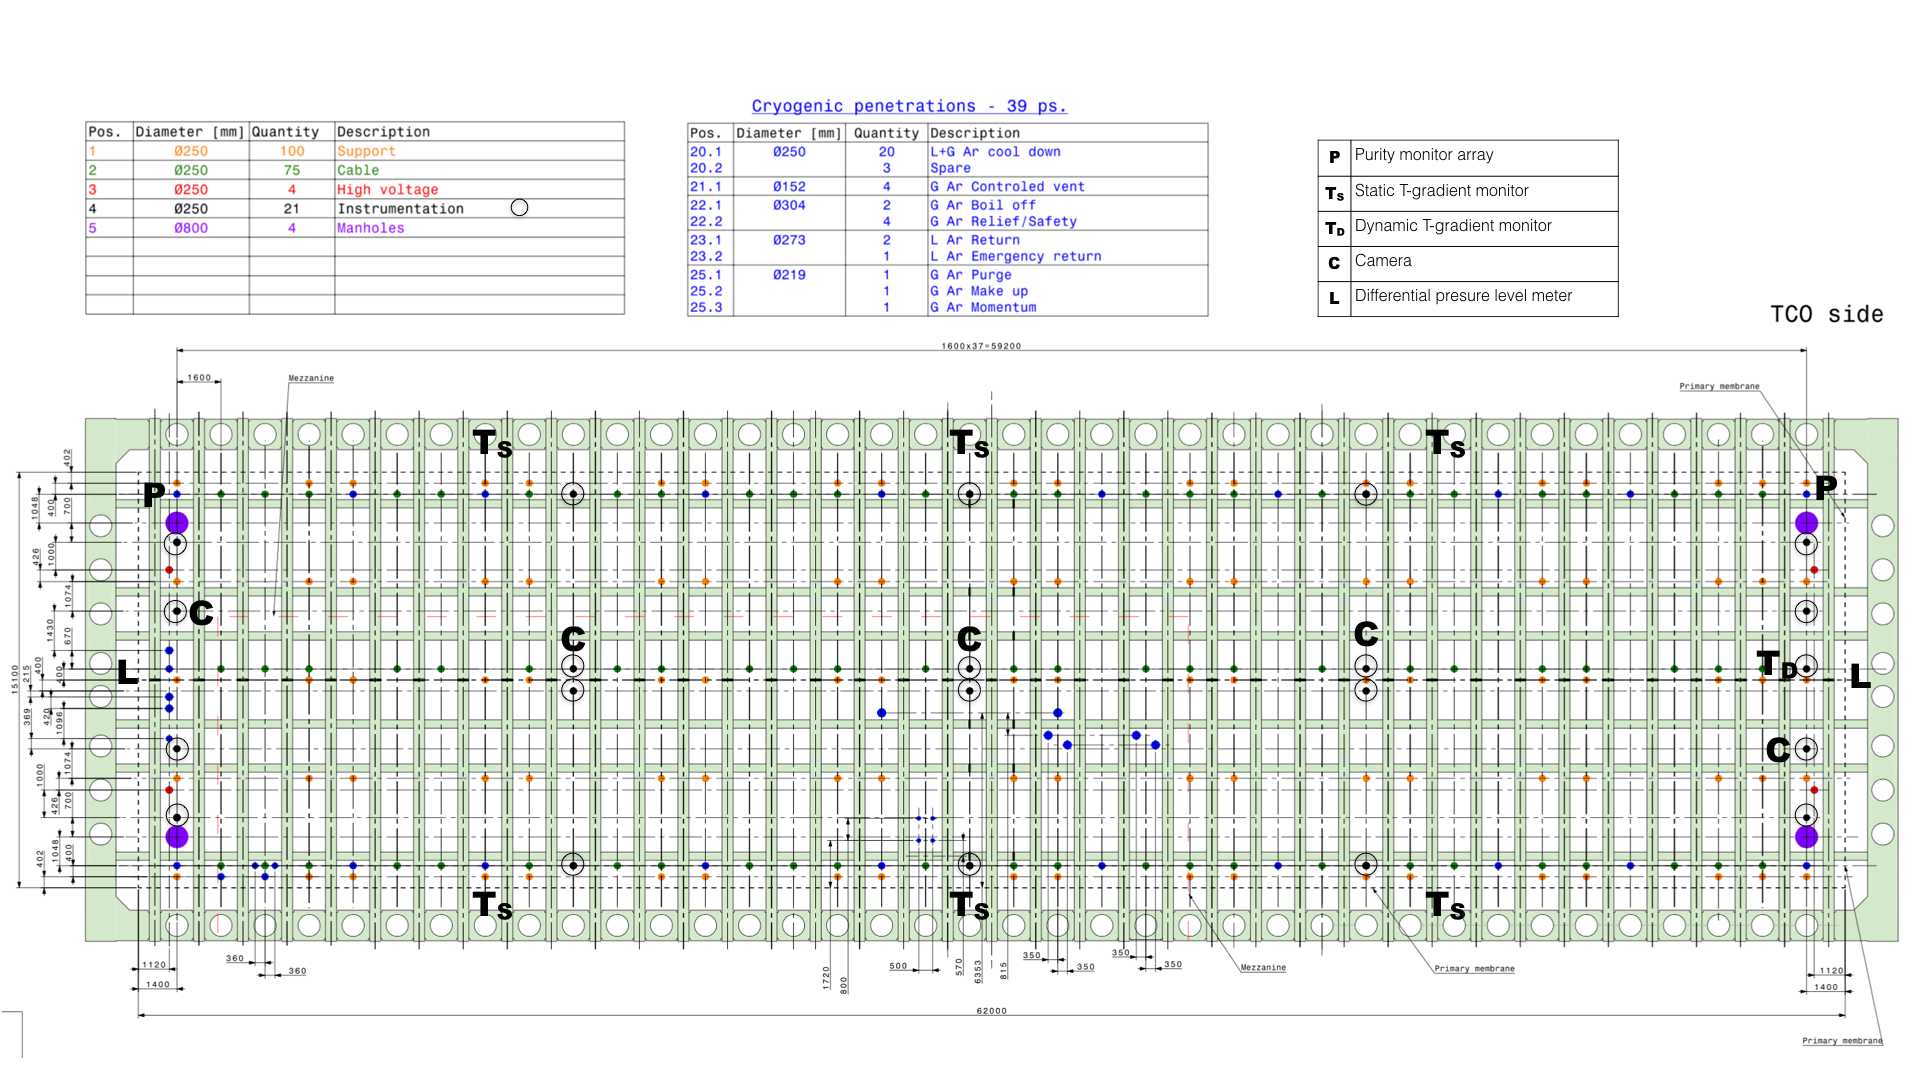
\includegraphics[width=0.95\textwidth]{cisc_cryostat_ports.png}
\end{dunefigure}




%%%%%%%%%%%%%%%%%%%%%%%%%%%%%%%%%%%
\subsection{Fluid Dynamics Simulations}
\label{sec:fdgen-slow-cryo-cfd}
% P. Strons
Proper placement of purity monitors, thermometers, and liquid level monitors within the detector module requires knowledge of how LAr behaves within the cryostat in terms of its fluid dynamics, heat and mass transfer, and distribution of impurity concentrations. 
Fluid motion within the cryostat is driven primarily by small changes in density from thermal gradients, although pump flow rates and inlet and outlet locations also contribute. 
Heat sources include exterior heat from the surroundings, interior heat from the electronics, and pump inlet temperature. 
The fluid flow behavior can be determined through simulation of LAr flow within the detector using ANSYS CFX, a commercially available Computational Fluid Dynamics (CFD) code. Such a model must include proper definition of the fluid characteristics, solid bodies and fluid/solid interfaces, and a means for measuring contamination, while still maintaining reasonable solve times.
Although simulation of the detector module presents challenges, there exist acceptable simplifications for accurately representing the fluid, the interfacing solid bodies, and variation of contaminant concentrations. Because of the magnitude of thermal variation within the cryostat, modeling of the LAr is simplified through use of constant thermophysical properties, calculation of buoyant force through use of the Boussinesq Model (using constant a density for the fluid with application of a temperature dependent buoyant force), and a standard shear stress transport turbulence model. Solid bodies that contact the LAr include the cryostat wall, the cathode planes, the anode planes, the ground plane, and the field cage. As in previous CFD models of the 35 ton cryostat and proto-DUNE by South Dakota State University (SDSU)~\cite{docdb-5915}, the field cage planes, anode planes, and ground plane can be represented by porous bodies. Since impurity concentration and electron lifetime do not impact the fluid flow, these variables can be simulated as a passive scalars, as is commonly done for smoke releases~\cite{cfd-1} in air or dyes released in liquids.
Significant discrepancies between real data and simulations can have potential impact on detector performance, as simulation results contribute to locating sensors and monitors, as well as defining various calibration quantities. However, methods of mitigating such risk include well-established convergence criteria, sensitivity studies, and comparison to results of previous CFD simulation work by SDSU and FNAL. Additionally, the simulation will be improved with input from temperature measurements and validation tests until the required agreement is achieved. An example of temperature distribution at one of the LAr inlet and outlets planes is shown in Fig. ~\ref{fig:cfd-example}. 



%%%%% Must find better pictures. Just use this for now
\begin{dunefigure}[cfd example]{fig:cfd-example}
  {Distribution of temperature at the outlet (left) and inlet (right) z positions, as predicted by SDSU CFD simulations (from ~\cite{docdb-5915}). }
  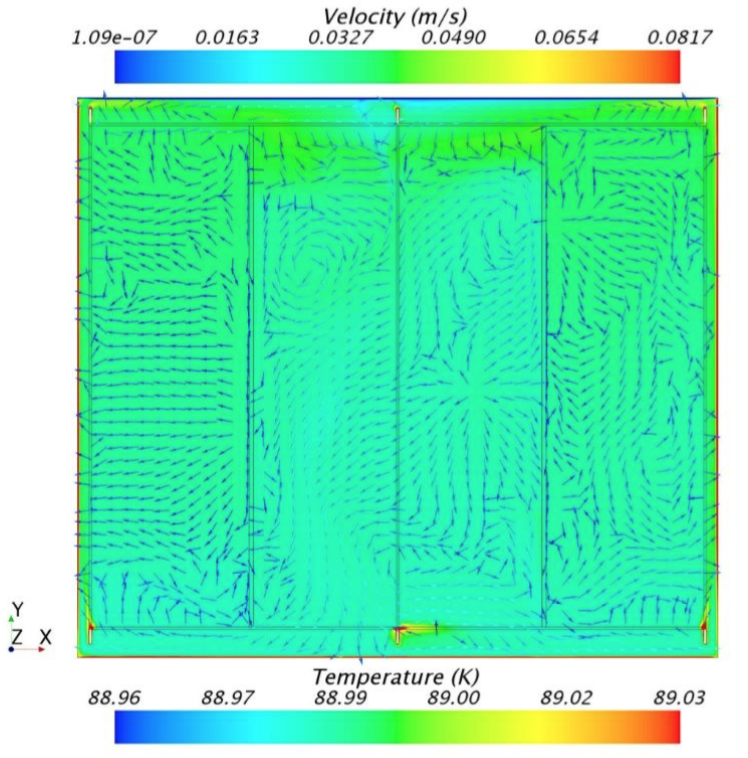
\includegraphics[height=0.4\textwidth]{cisc_cfd_outlet_z0.png}
  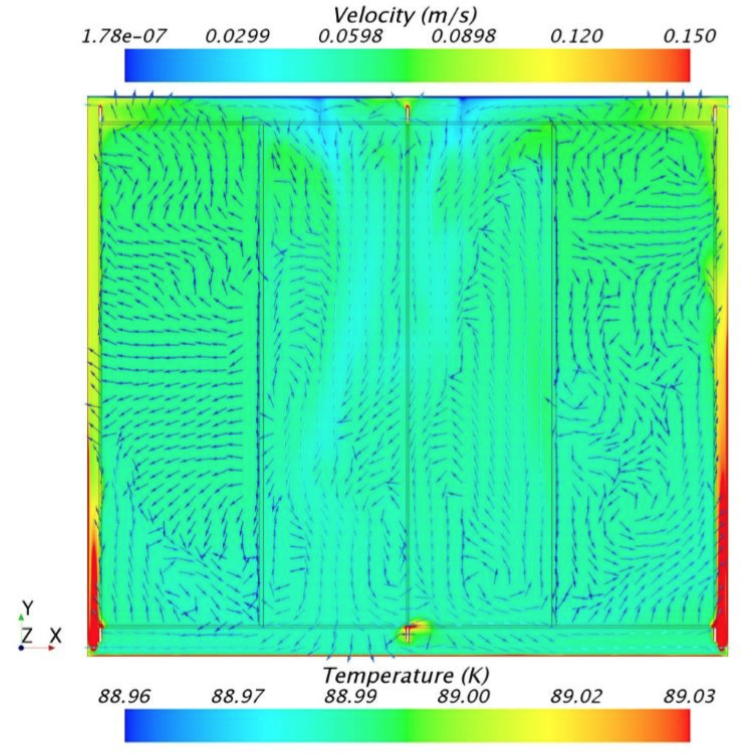
\includegraphics[height=0.4\textwidth]{cisc_cfd_inlet_z52.png}
\end{dunefigure}


  
